\documentclass[a4paper]{article}
\usepackage{amsmath}
\usepackage{amssymb}
\usepackage{geometry}
\usepackage{natbib}
\usepackage{float}%稳定图片位置
\usepackage{graphicx,subfig}%画图
\usepackage{caption}
\usepackage[english]{babel}
\usepackage{indentfirst}%缩进
\usepackage{enumerate}%加序号
\usepackage{multirow}%合并行
\usepackage{hyperref}
\usepackage{verbatim}
\usepackage{geometry}%设置页边距
\geometry{top=0.5in,bottom=0.5in,left=0.5in,right=0.5in}
\begin{document}
\begin{center}
    \Large{\textbf{SI618 Individual Project Report}}\\
    \large{Chongdan Pan $\bullet$ pandapcd $\bullet$ pandapcd@umich.edu}
\end{center}
\section{Motivation}
Recently, cryptocurrencies like Bitcoins have become the hottest topic all over the world. Cryptocurrencies are being used in multiple areas including decentralized finance, application development, art collections, and etc. The market value also increased dramatically in the past 10 years, from less than one hundred dollars to more than two trillion dollars.

\par To make a profit, many people and organizations are getting involved in this area. There is news that Grayscale, an investment institution, owns cryptocurrencies assets worth more than 20 billion dollars. Through mobile trading applications like PayPal, it’s easy for even normal people or retail investors to buy and trade cryptocurrencies at any time. However, such a low entry barrier and mania also implies high risk. Investors can make a great fortune thanks to the 10 times increment of price in less than half of one year, but there is also news that people lose a family fortune because the price may plummet 50\% in 10 hours.

\par To get an insight into cryptocurrencies, especially for retail investors, this project aims at achieving the following goals:
\begin{itemize}
    \item Calculate, analyze, and compare the previous trading data and specific features of some cryptocurrencies and other typical indexes like S\&P 500 or 10-year treasury to get a general idea of their price movement.
    \item Simulate simple trading strategies suitable for retail investors and calculate the return and features of these strategies.
    \item Try to find the pattern or relationship between cryptocurrencies and other typical indexes.
\end{itemize}

\section{Data Source}
Market data from Binance and Yahoo Finance will be used in this project. The first one is the four-hour market data of Bitcoin and Ethereum retrieved from the Binance Restful API from Jan.1st, 2018 to Oct.15th, 2021. The second one is US 10-year treasury, S\&P 500, NASDAQ, and gold price trend from Yahoo Finance.
\begin{itemize}
    \item Binance has a lot of public REST API providing cryptocurrencies’ historical market data of different frequencies at different times. \href{https://binance-docs.github.io/apidocs/spot/en/#market-data-endpoints}{(https://binance-docs.github.io/apidocs/spot/en/\#market-data-endpoints)}. The API will accept Http Get requests with certain parameters, and return at most 1000 periods' market data in json (e.g. \href{https://api.binance.com/api/v3/klines?symbol=ETHUSDT\&interval=4h}{https://api.binance.com/api/v3/klines?symbol=ETHUSDT\&interval=4h}).
    \par The data are well-structured in 8304 rows and 12 columns. Each row represents one four-hour period during the time interval, and each column represents one following field in this period:
    \begin{itemize}
        \item OpenTime (int): The start time of the four-hour period in epoch time
        \item Open (float): The open price
        \item High (float): The highest price
        \item Low (float): The lowest price
        \item Close (float): The close price
        \item TradeVolume (float): The total trade volume
        \item CloseTime (int): The end time of the four-hour period in epoch time
        \item TradeValue (float): The quote asset volume
        \item TradeCount (int): The number of trades
        \item BuyVolume (int): The total volume of trades activated by buyers
        \item BuyValue (float): The quote asset volume of trades activated by buyers
        \item Useless (int): An ignored field
    \end{itemize}
    \item Yahoo Finance will be used to fetch daily market data of traditional index or assets including US 10-year treasury, S\&P 500, NASDAQ, and gold price for comparison and reference. The user can get the data in CSV form after inputting the asset symbol and period. (\href{https://query1.finance.yahoo.com/v7/finance/download/%5EIXIC?period1=1483228800&period2=1634256000&interval=1d&events=history&includeAdjustedClose=true}{https://query1.finance.yahoo.com/v7/finance/download/\%5EIXIC?period1\\=1483228800\&period2=1634256000\&interval=1d\&events=history\&includeAdjustedClose=true}). Unlike Binance’s datasets, Yahoo’s data has 954 rows and 7 fields, which are:
    \begin{itemize}
        \item Date (string): The date of the data
        \item Open (float): The open price
        \item High (float): The highest price
        \item Low (float): The lowest price
        \item Close (float): The close price 
        \item Adj Close (float): The adjusted close price due to exit right or other reasons
        \item Volume (int): The total trade volume
    \end{itemize}
\end{itemize}
\section{Data Manipulation}
\begin{figure}[H]
    \centering
    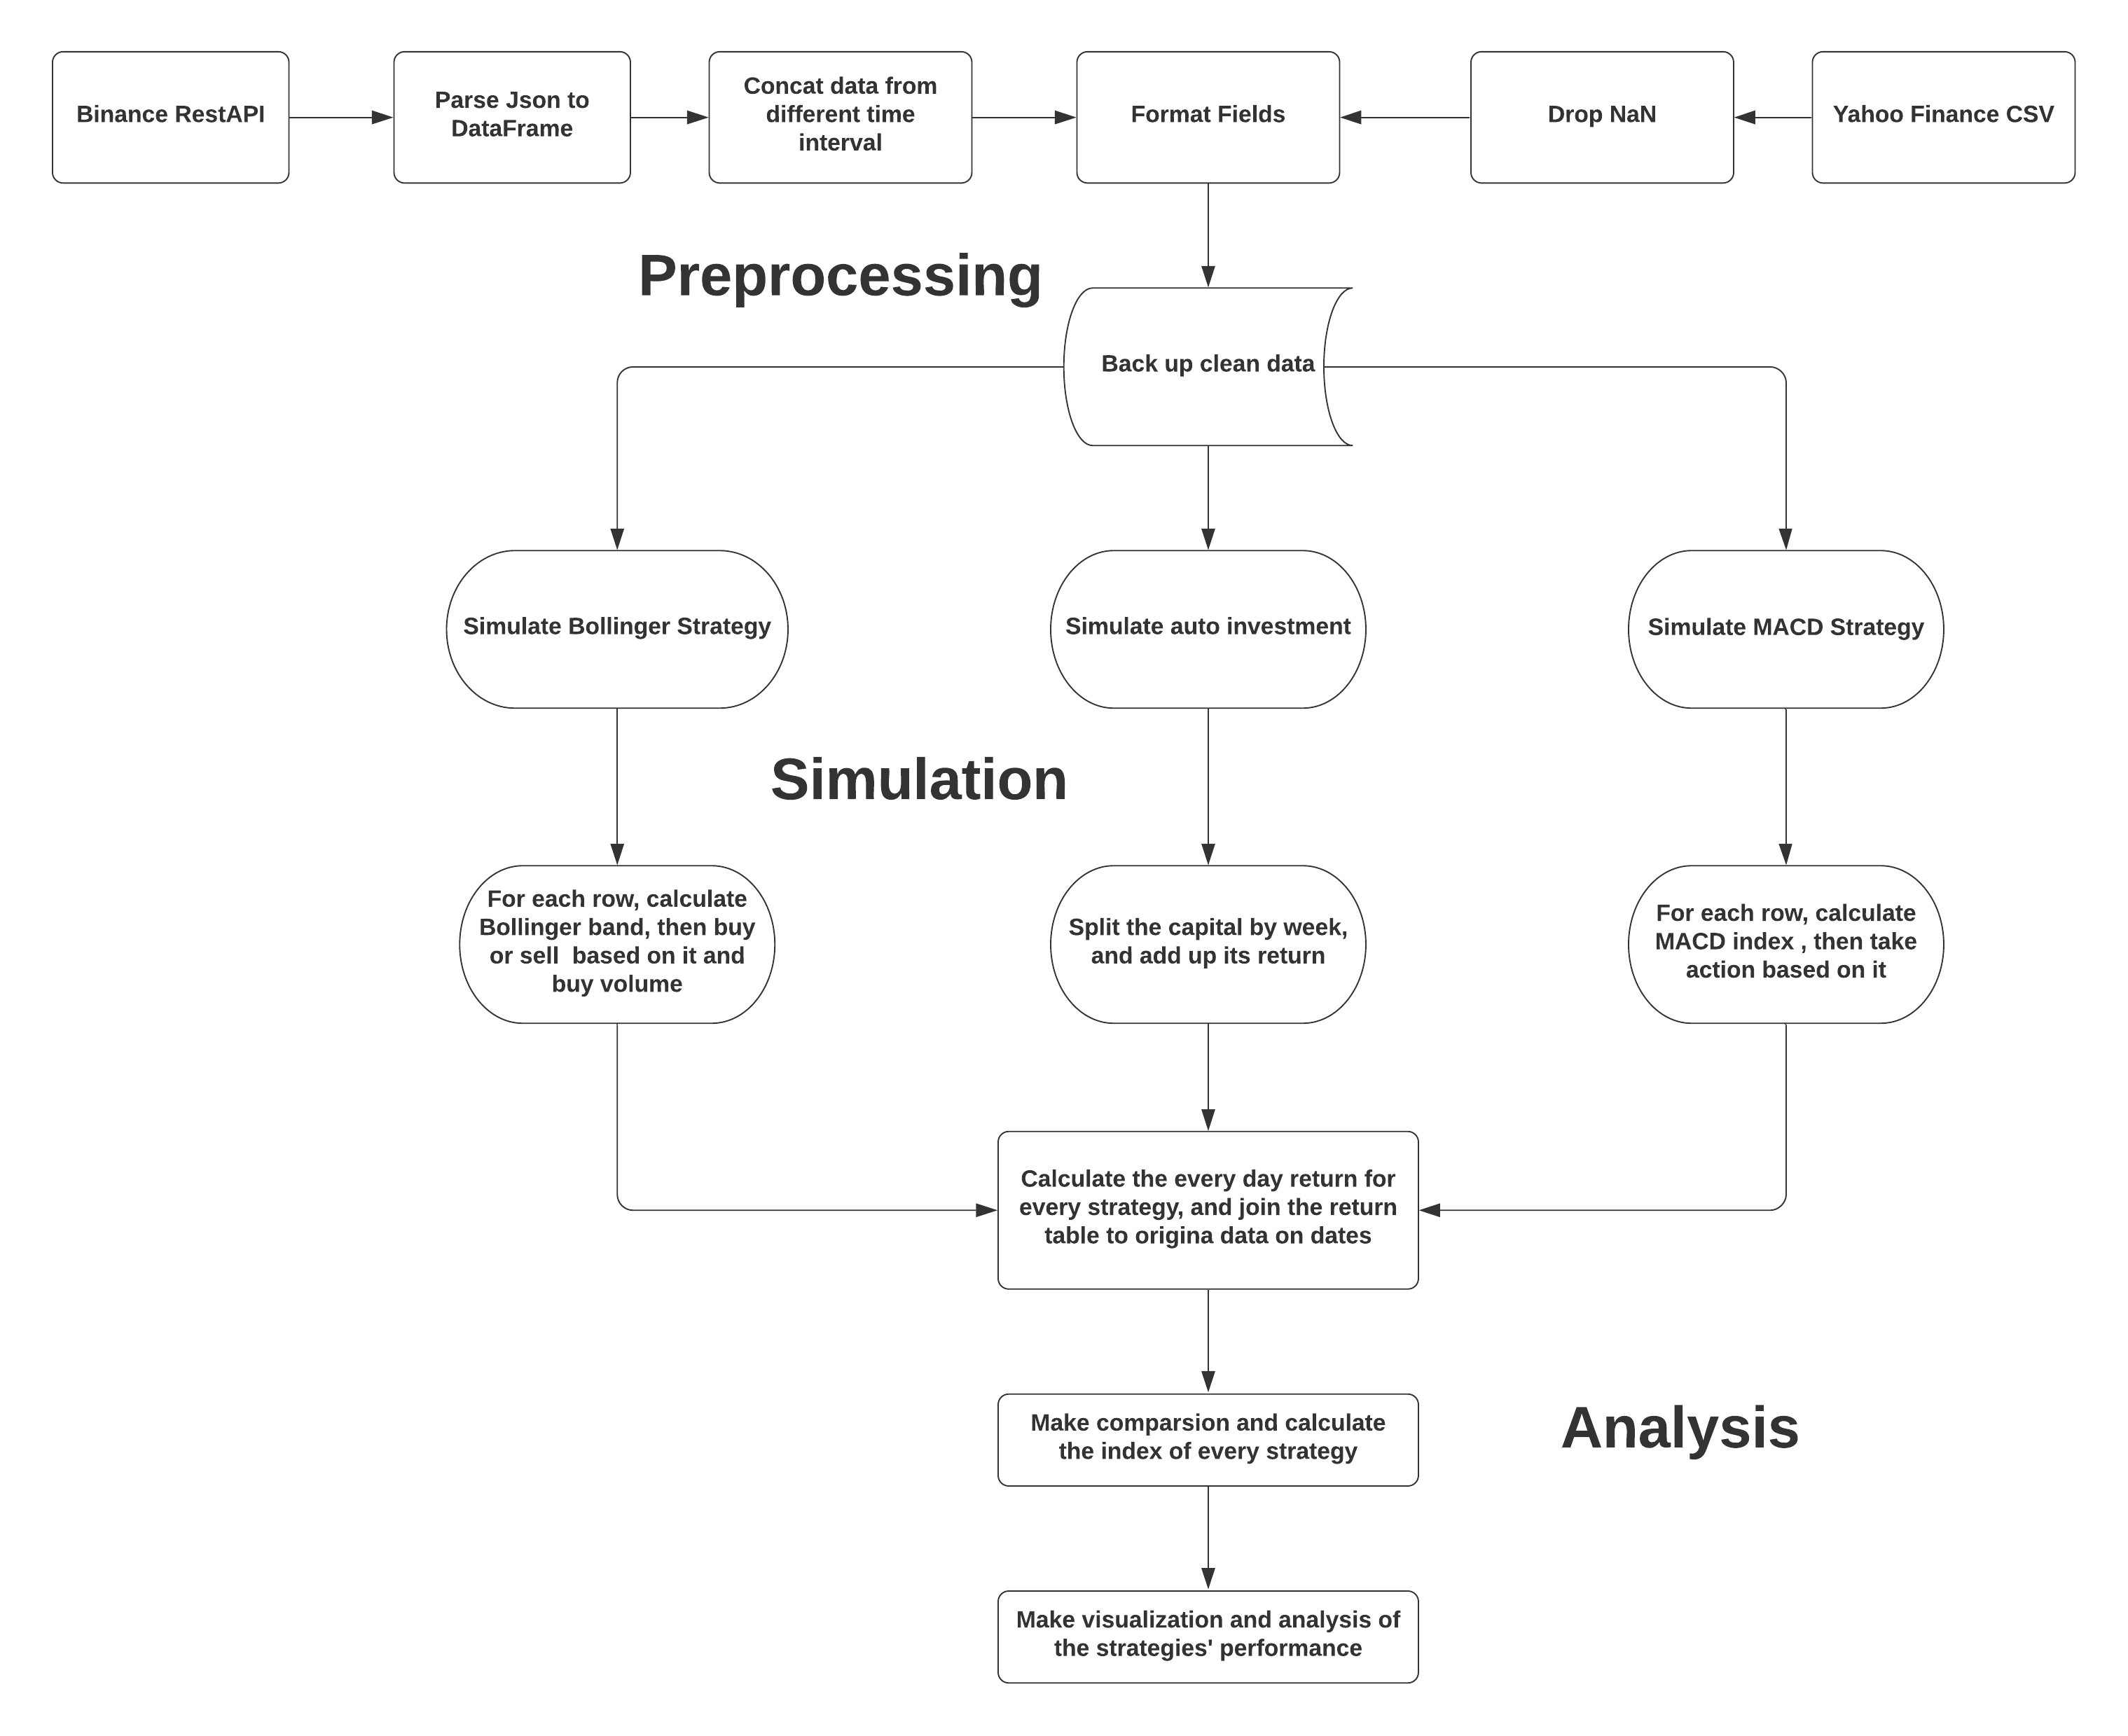
\includegraphics[scale=0.5]{Flowchart.png}
    \caption{Flowchart of the manipulation and analysis}
\end{figure}
The data manipulation will have three parts including preprocessing, simulation, and analysis. The source code of each part will be coded in one python file, and the data frame will be saved as well by the end of each part. 
\par Notice that the manipulation will all be conducted in Spark 3.2's PySpark API. The latest 3.2 version provides pandas with new features, which are extremely helpful and efficient for the user to perform manipulation which is difficult to make in an old version. In addition, according to the document provided by DataBricks, the pandas API provided by Spark has a much better performance than the original one.
\par Unlike a common map-reduce job, this is project has some calculations in time-series, which can only be conducted in a certain order rather than parallelly. However, Spark still plays an important role in it and all data are stored based on RDD so that the project can be conducted on a cluster as well.
\subsection{Preprocessing}
The preprocessing including concatenation, standardizing the fields, as well as drop the incorrect data. 
\begin{itemize}
    \item Since the user can only fetch data of at most 1000 periods (rows) at one time from Binance, all these rows needed to be concatenated together in chronological order for every asset.
    \item After concatenation, another new field call "Dates" will be set as the date difference between the row's date or timestamp and the first date, which is Jan.1st, 2018. This field will be used to order and match the daily data in chronological order because cryptocurrencies and traditional assets have different trading hours. \\
    This API used here is slightly different from pandas API because it returns float rather than pd.Timedelta
    \begin{verbatim}
df["Dates"] = (ps.to_datetime(df["TimeStamp"]) - ps.to_datetime("20180101")) // 86400
    \end{verbatim}
    \item Rows with NaN will be dropped from the datasets since they provide no help for the trading.
    \item Then some fields of the data will be discarded because they're not all used by the simple strategies. The discarded fields are OpenTime, CloseTime, TradeValue, TradeCount, TradeVolume, Volume, BuyValue, Useless, Adj Close, and Date.  
\end{itemize}
\subsection{Strategy Simulation}
In this project, the trading strategies to be simulated will be simple enough for the retail investors to execute. For simplicity, the strategies will not make action related to shorting and the trading service fee will be ignored as well. 
\par Since the simulation is conducted chronologically, the dataset must be iterated orderly to produce the real signal for every strategy, and each strategy will be implemented as a function for iteration of the dataset.
\begin{verbatim}
signal = strategy(df, asset_type) # call the strategy
revenue = spark.createDataFrame(signal, schema="Cash FLOAT, Num FLOAT, \ 
Revenue FLOAT, Dates FLOAT")
revenue.registerTempTable("Revenue")
df.to_spark().registerTempTable("{}_df".format(strategy.__name__))
sql = "SELECT Close, Revenue.Revenue as Revenue, Revenue.Dates as Dates FROM {name}_df\
JOIN Revenue ON {name}_df.Dates=Revenue.Dates".format(name=strategy.__name__)
df = sqlContext.sql(sql)
\end{verbatim}
\par After the iteration, a new Spark data frame will be created including the return, and they'll be further joined by the "Dates" column. Based on retail investors' ability, their strategies will make trade decisions once every day.
\subsubsection{Automatic Invesment}
This is a simple strategy recommended by Warren Buffett, which has been proved to be effective on long-term investment. In this strategy, investors will invest a fixed amount of money into the asset in each period no matter what's the price. There are 198 weeks in this simulation, so there will be 198 trades, and the final net value will be calculated based on the final close price.
\subsubsection{MACD}
MACD is a very famous technique indicator used in trading. It first gets DIF by calculating the difference of two exponential moving average values of price in two different periods.  Then another exponential operation will be conducted on the DIF again and generate a new value called DEA. The difference between DIF and DEA will be used as the trading signal in this strategy. In this project, the two periods for DIF calculation will be 13 and 26 days, and the period for the second calculation will be 9 days. The strategy will buy the asset when the difference between DEA and DIF first turns positive from negative, and sell it vice versa. Since the cryptocurrency's data is in a 4-hour frequency, the calculation will be slightly different from the index. During the simulation, the performance of the strategy will be calculated as the sum of cash the assets with close price at that time.
\subsubsection{Bollinger Band with Volume}
Bollinger band is another technical indicator created based on one exponential moving average of price and its standard deviation in a certain period. This project will set the period as 13 days. The new rolling feature in Spark 3.2 will be used to calculate the standard deviation.
\begin{verbatim}
df["Close"].rolling(162).std()
\end{verbatim}
\par The upper band and lower band will be calculated based on plus two times standard deviation to the average price or minus two times the standard deviation from it. To improve the return, buy volume is another requirement for the trade, and its exponential moving average is calculated as well. The strategy will buy the asset when the buy volume is extremely higher than 1.5 times its ema as well as the price comes up across the lower band. When the price comes down to cross the upper band, the strategy will sell all assets no matter what the buy volume is.
\par Note that this strategy can only be applied to cryptocurrencies because indexes don't have a buying volume.
\subsection{Postprocessing}
When the simulations are completed, the result will be joined by the dates because cryptocurrencies’ are traded 24 hours and the trading decisions are made every 4 hours in the simulation, while for the traditional assets, the trading can only be made on workdays. To align the simulation, the data of traditional assets will be merged with the data of cryptocurrencies. For PySpark, it's easier to directly use the data frame's API rather than write a SQL query because the user doesn't need to be worried about the duplicate columns.
\begin{verbatim}
ans = strategy.join(price, ["Dates"]).orderBy(["Dates"], how="left")
\end{verbatim}
After the data are joined, there will be missing value for the traditional assets on days when these assets are not traded. These data will be filled by the previous data because future information is prohibited in time-series analysis. It happens that the traditional data also has no information on the first day of the simulation, hence this day is removed as well. 
\begin{verbatim}
ans = ans.to_pandas_on_spark().fillna(method="ffill").iloc[1:]
\end{verbatim}
\section{Analysis and Visualization}
In total, there will be fourteen simulations upon three strategies and six assets, the performance of each strategy will be saved and representation visually through Altair.
\subsection{From the perspective of price, what's the difference between cryptocurrencies and other assets.}
No strategy will be simulated at this stage because a general understanding of the asset is usually essential for investment. A good way for this is to make a comparison. Normalization will be performed upon every asset first so that they have the same initial price value 1. This is done through SparkSQL.
\begin{verbatim}
sql = "SELECT {asset}_df.Dates as Dates, Close / start as {asset} FROM {asset}_df \
    CROSS JOIN (SELECT Close as start FROM {asset}_df ORDER BY Dates LIMIT 1) AS tmp".
price[asset] = sqlContext.sql(sql.format(asset=asset)).dropDuplicates(["Dates"])
\end{verbatim}
When all asset is normalized and joined together, Altair is used to plot an interactive chart of the movement of each asset.
\begin{figure}[H]
    \centering
    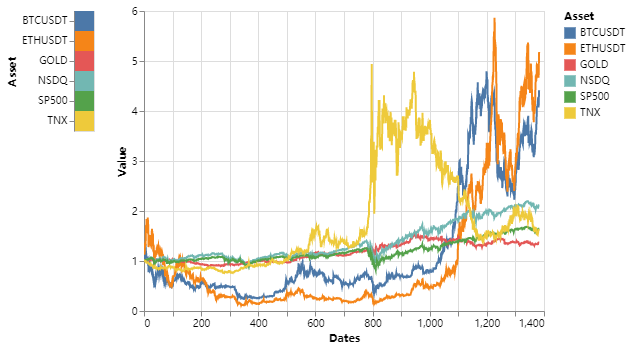
\includegraphics[scale=0.5]{Q1.png}
    \caption{Price movement of different assets in three years}
\end{figure}
The visualization shows that BTC, ETH, and TNX have a larger fluctuation range than other assets. For the cryptocurrencies’ including BTC, ETH, they share a similar movement of their price. As shown in the chart, the investors will have a significant return if they can hold the cryptocurrencies for a long time. To analysis the movement in a quantitative way, three indicators are used.
\begin{itemize}
    \item \textbf{Ret: } It's calculated by dividing the asset's last day's price by the asset's first day's price. It shows the earning ability of the asset. The return can be either calculated by SparkSQL or pandas on Spark.
\begin{verbatim}
sql = "SELECT {asset}_df.Close / tmp.Close FROM {asset}_df CROSS JOIN (SELECT \
    Close FROM {asset}_df ORDER BY Dates LIMIT 1) AS tmp ORDER BY Dates DESC LIMIT \
    1".format(asset=asset)
\end{verbatim}
    \item \textbf{Std: } It's calculated as the standard deviation of the asset's price during the three years. A higher standard typically implies higher volatility, which means it's harder for the investor to find a good opportunity to buy or sell the asset. The standard deviation can be calculated easily through SparkSQL
\begin{verbatim}
sql = "SELECT STD(Close) FROM {asset}_df".format(asset=asset)
\end{verbatim}
    \item \textbf{Maximum Drawdown: } Drawdown is a term defined by the ratio of current price over the previous highest price, while the maximum drawdown can represent the highest risk that the investor must stand. This indicator is very useful because it's usually hard for one to hold the asset during a drawdown, especially for retail investors who're very afraid of loss. This indicator is easier to calculate through pandas on Spark due to the cummax method.
\begin{verbatim}
max_drawdown = (1 - ans[column] / ans[column].cummax()).max()
\end{verbatim}
\end{itemize}
\begin{table}[H]
    \centering
    \begin{tabular}{@{}|c|c|c|c|@{}}
    \hline
    asset   & return & max drawdown & std   \\ \hline
    BTC & 4.43   & 0.8          & 1.161 \\ \hline
    ETH & 4.60   & 0.94         & 1.27  \\ \hline
    GOLD    & 1.37   & 0.18         & 0.19  \\ \hline
    NSDQ    & 2.16   & 0.3          & 0.38  \\ \hline
    SP500   & 1.65   & 0.34         & 0.21  \\ \hline
    TNX     & 1.62   & 0.71         & 1     \\ \hline
    \end{tabular}
\end{table}
\par The indicator shows similar information as the charts, where the cryptocurrencies’ have much higher volatility as well as a return than traditional assets.
\subsection{Whether cryptocurrencies are a good investment asset for retail investors? If so, how should they make an investment?}
Indeed, it's extremely hard for retail investors to buy an asset and hold it for years because they're very restless and eager to make profits as soon as possible. Therefore, the simulation result is very important for them to know what's the best way to invest.
\par Similar to the price analysis, return, maximum drawdown, and the standard deviation are calculated. What's more, two more typical indicators for fund analysis are calculated to evaluate the strategy's performance.
\begin{itemize}
    \item \textbf{Sharp Ratio: } Sharp ratio is very typical to evaluate the strategy's return ability based on each risk taken by the investors. It's calculated by the difference between return and risk-free rate divided by the standard deviation. Since the data is limited in this project, the risk-free rate is set as one.
    \item \textbf{Carmer Ratio: } Carmer ratio is a modified version of the Sharp Ratio. It's calculated by dividing the return by the maximum drawdown. To retail investors, their risk tolerance is more expressed in the maximum drawdown that they can take rather than the standard deviation.
\end{itemize}
When the strategy is making a profit, the higher these two indicators are, the better the performance is. 
\subsubsection{Automatic Investment}
\begin{figure}[H]
    \centering
    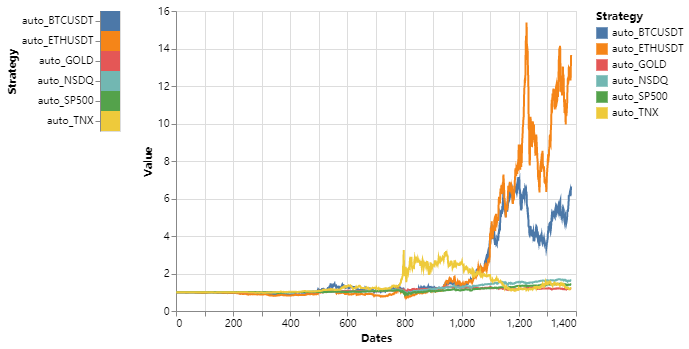
\includegraphics[scale=0.5]{Q2.png}
    \caption{Performance of automatic Investment}
\end{figure}
\begin{table}[H]
    \centering
    \begin{tabular}{@{}|c|c|c|c|c|c|@{}}
    \hline
    asset   & return & max drawdown & std & sharp ratio & carmer ratio \\ \hline
    BTC     & 6.64   & 0.53 & 1.66 & 3.39  & 10.6 \\ \hline
    ETH     & 13.6   & 0.59 & 3.32 & 3.8   & 21.4\\ \hline
    GOLD    & 1.19   & 0.15 & 0.09 & 1.99  & 1.85\\ \hline
    NSDQ    & 1.64   & 0.19 & 0.22 & 2.86  & 3.34\\ \hline
    SP500   & 1.42   & 0.21 & 0.14 & 3     & 2\\ \hline
    TNX     & 1.23   & 0.66 & 0.55 & 0.41  & 0.34\\ \hline
    \end{tabular}
\end{table}
The result shows that automatic investment is a good strategy for cryptocurrencies as well. The return is much higher and the maximum drawdown is also lower. What's more, compared to the traditional assets, the sharp ratio and the Carmer ratio of the cryptocurrencies’ are higher as well.
\par Even for other assets, the strategy also achieves a good performance because it can provide considerable profit with low risk. 
\subsubsection{MACD Strategy}
\begin{figure}[H]
    \centering
    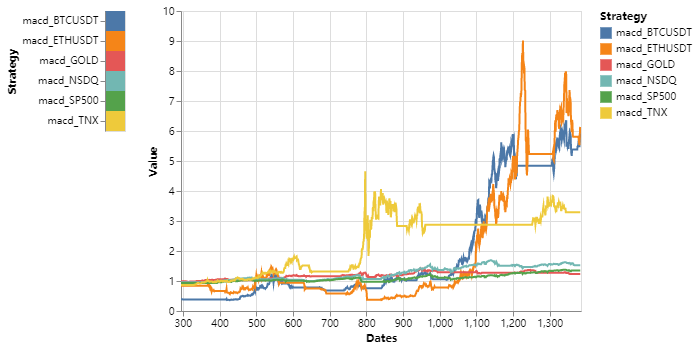
\includegraphics[scale=0.5]{Q3.png}
    \caption{Performance of MACD strategy}
\end{figure}
\begin{table}[H]
    \centering
    \begin{tabular}{@{}|c|c|c|c|c|c|@{}}
    \hline
    asset   & return & max drawdown & std & sharp ratio & carmer ratio \\ \hline
    BTC     & 6.07   & 0.68 & 1.72 & 2.95  & 7.49 \\ \hline
    ETH     & 5.58   & 0.8 & 1.83 & 2.5   & 5.72\\ \hline
    GOLD    & 1.24   & 0.13 & 0.13 & 1.9   & 1.85\\ \hline
    NSDQ    & 1.53   & 0.16 & 0.23 & 2.3   & 3.34\\ \hline
    SP500   & 1.35   & 0.15 & 0.12 & 2.83  & 2.39\\ \hline
    TNX     & 3.29   & 0.61 & 1    & 2.29  & 3.78\\ \hline
    \end{tabular}
\end{table}
The simulation shows that the MACD strategy is not so friendly to the high volatility as to the automatic investment strategy because its performance is worse than the automatic investment strategy, while there is not so much difference for traditional assets. It even plays extremely well for the TNX. However, the strategy does do a good job, because the return is still higher than no strategy. 
\par To dig out more insight into the strategy, the information about each trade is collected as well. The number of trades and the average profit of the trades are calculated. The win rate is calculated as well, which means the proportion of the trades that gain profit. Notice that the strategy does fewer trades than the automatic strategy, which means a lot of service charges will be saved, but this part is not taken into consideration in this project.
\begin{table}[H]
    \centering
    \begin{tabular}{@{}|c|c|c|c|@{}}
    \hline
    asset   & trade number & win rate & average profit \\ \hline
    BTC & 16   & 0.438          & 0.323 \\ \hline
    ETH & 11   & 0.545         & 0.476  \\ \hline
    TNX & 9   & 0.44          & 0.254 \\ \hline
    NSDQ & 11   & 0.545        & 0.048  \\ \hline
    SP500 & 10   & 0.4        & 0.035 \\ \hline
    GOLD & 10   & 0.5         & 0.023 \\ \hline
    \end{tabular}
\end{table}
\begin{figure}[H]
    \centering
    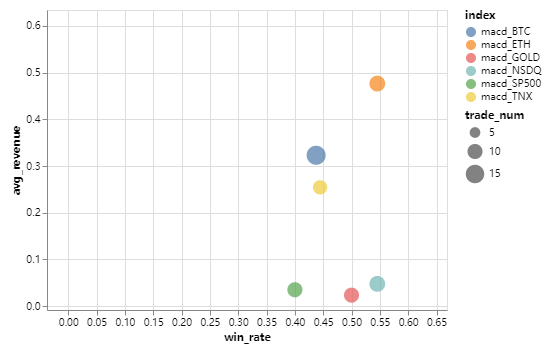
\includegraphics[scale=0.5]{Q4.png}
    \caption{Performance of MACD strategy}
\end{figure}
The high average profit in the table and visualization shows that the strategy can typically catch a good opportunity where it can make a huge amount of profit. However, it also catches some bad opportunities where it loses money. If a filter can be applied, then it'll have a better performance.
\subsubsection{Bollinger Strategy}
\begin{figure}[H]
    \centering
    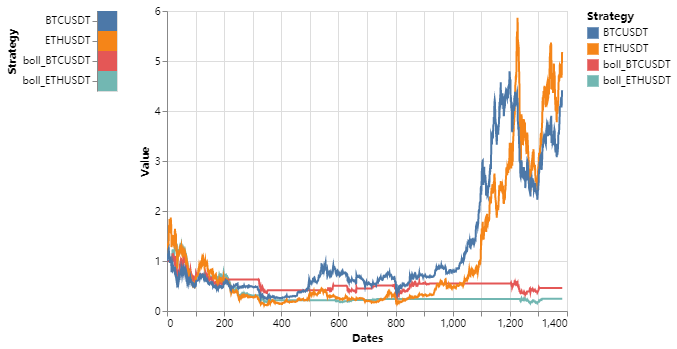
\includegraphics[scale=0.5]{Q5.png}
    \caption{Performance of Bollinger strategy}
\end{figure}
\begin{table}[H]
    \centering
    \begin{tabular}{@{}|c|c|c|c|@{}}
    \hline
    asset   & return & max drawdown & std \\ \hline
    BTC & 0.46   & 0.76          & 0.13 \\ \hline
    ETH & 0.24   & 0.89         & 0.23  \\ \hline
    \end{tabular}
\end{table}
The simulation shows that the Bollinger strategy can't even make any profit from cryptocurrencies in a long term. That's because the strategy usually sells the asset before the main rise of the price. On the other hand, it also buys the asset before the reverse of the price. The strategy ignores the huge momentum of cryptocurrencies’ so it always buys and sells the assets too early. 
\subsection{Is there any relation between cryptocurrencies and other assets?}
The correlation between two type of assets can be calculated by SparkSQL in the following way
\begin{verbatim}
corr = price.corr("ETHUSDT", "BTCUSDT")
\end{verbatim}
\begin{figure}[H]
    \centering
    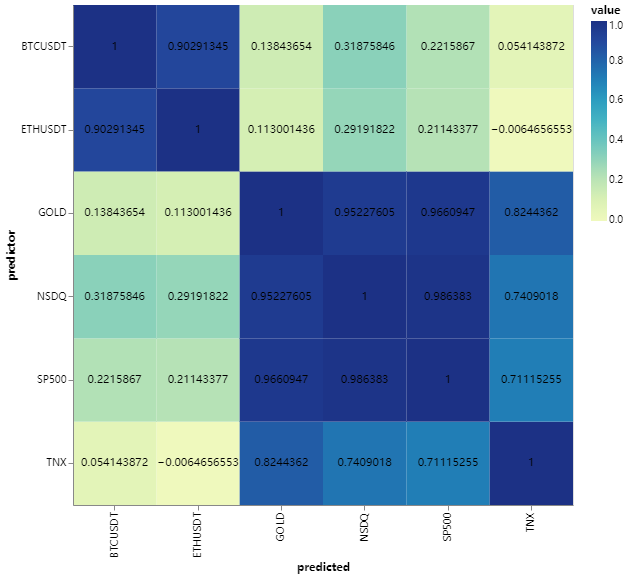
\includegraphics[scale=0.4]{Q6.png}
    \caption{Correlation of different asset}
\end{figure}
According to the heatmap created for the correlation, there is an obvious relation within the cryptocurrencies or the traditional assets, but the relation between these two markets is quite subtle. For the correlation between these two markets, the correlation between NASDAQ and BTC is highest. It's probably they're about the newest technology. Although the result implies it's hard to predict the price of one market through another, it does reflect the possibility to predict one asset through another in the same market. However, to make a prediction, future information is prohibited. Therefore, the predicted value is shifted in the time series for the prediction. In the following chart, each value represents the correlation between the column asset's price and the row asset's price on the last date.
\begin{verbatim}
w = Window().partitionBy().orderBy(col("Dates"))
predict_price = price.withColumn("predict", lag(asset, 1).over(w))
corr = predict_price.corr("predict", predicted_asset))
\end{verbatim}
\begin{figure}[H]
    \centering
    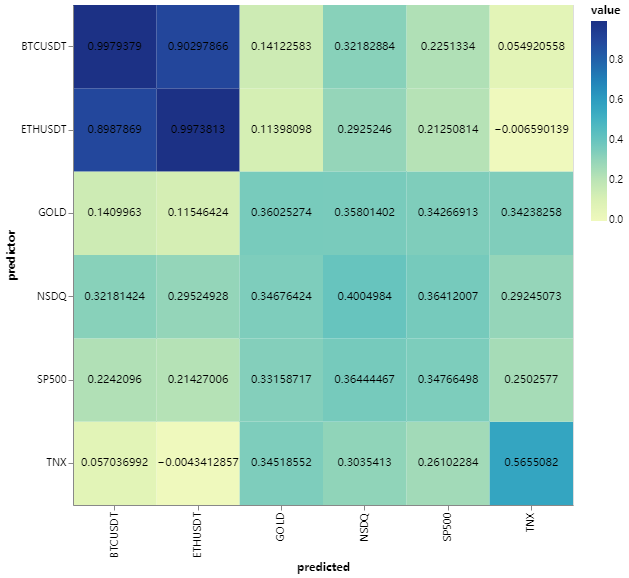
\includegraphics[scale=0.4]{Q7.png}
    \caption{Future correlation of different asset}
\end{figure}
According to the heatmap created for the future correlation, the correlation within the cryptocurrencies market is more obvious than it in a different market. It seems the best way to predict the price is to use the previous information from the market itself.
\subsection{Conclusion}
This analysis can provide the viewers with a general understanding of cryptocurrencies and other traditional assets. Cryptocurrencies have a higher fluctuation range and higher return. It turns out the key to success in this market is patience because the price rise very quickly, however, the price may decline at an astonishing speed as well and the investor may be too afraid of loss so that they will sell the asset at a low price rather than keep it.
\par Through the simulation, it turns' out Warren Buffett's automatic investment strategy still works very well in the cryptocurrencies market. It may be because it reduces the impact of the high volatility. The typical MACD strategy achieves a considerable return. However, the Bollinger strategy is not very competitive in this market, because it's always too impatient. It's more similar to retail investors' behavior than the other two strategies.
\par As for the correlation, it turns out that the correlation within the cryptocurrencies market is much higher than others. So the best choice is to make a prediction based on the market itself.
\section{Challenges and Limitations}
There are many challenges in this project. The first challenge is due to the diversity of the data
Since the data are from different sources, a lot of preprocessing is required including renaming the fields and concatenating them. In addition, since the assets are traded at different times, these data need to be realigned and joined together.
\par The second challenge is that it's hard to decompose a time-series analysis into a map-reduce or parallel computing job because every computation needs the result from the last one. Therefore, iteration is inevitable in this project. However, there are still many scenarios where Spark's features can be used. For example, SparkSQL is used for the normalization as well as the join stage. In addition, the new feature "pandas on Spark" provided in the latest 3.2 version are helpful, especially for cumulative computation. Such features make it possible and efficient to perform basic pandas operations on Spark or large computation systems.
\par However, it must be admitted that there are many limitations to this project. First, the simulation ignores many factors that may affect the performance of the strategy, such as the service charge for trade. Second, the strategies used for simulation are extremely simple, and many fields are not being used. For example, the trade volume can provide a lot of information for trading. In addition, many parameters used in these strategies and indicators are not well-turned, so the performance and evaluation are affected. What's more, the assets and strategies used for this project are also limited, because there are tons of different assets which can be used to generate an investment strategy. Especially for the TNX, this project does an external reverse operation on its value, and that's not the typical way how it works in a real market. That may explain why the treasury bond can have such a return, which is impossible.
\par Further improvements can be made in many aspects. For example, the strategy can be designed based on the cross-section of the market rather than the time series so that it can take full advantage of the feature of Spark. 
\end{document}